\documentclass[tikz]{standalone}

\usepackage{tikz}
\usetikzlibrary{automata}

\begin{document}

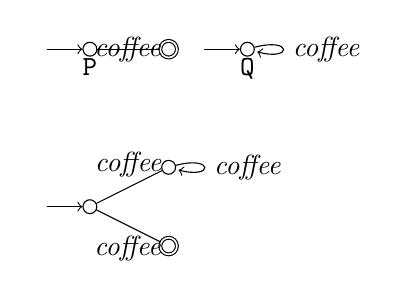
\begin{tikzpicture}
    \tikzstyle{every state}=[
        draw,
        shape=circle,
        inner sep=1pt,
        minimum size=5pt,
        final/.style={double,minimum size=6pt},
        initial text=] 

    [->,auto,node distance=1.5cm]
    \renewcommand{\a}[1]{\textit{#1}}
    \node[state,initial] (a0) {}; 
    \node[state, final, right of=a0] (a1) {};
    \node[state,initial,right of=a1] (b0) {}; 
    \node[state,initial,below of=a0,yshift=-1cm] (n0) {}; 
    \node[state, right of=n0,yshift=0.5cm] (n1) {}; 
    \node[state,final,right of=n0,yshift=-0.5cm] (n2) {};
    \path (n0) edge node[above]{\a{coffee}} (n1) edge node[below]{\a{coffee}} (n2)
            (n1) edge[loop right] node{\a{coffee}} (n1)
            (a0) node[below]{\ttfamily P} (a0) edge node{\a{coffee}} (a1)
            (b0) node[below]{\ttfamily Q} (b0) edge[loop right] node{\a{coffee}} (b0);
\end{tikzpicture}
\end{document}